%%%%%%%%%%%%%%%%%%%%%%%%%%%%%%%%%%%%%%%%%%%%%%%%%%%%%%%%%%%%%%%%%%%%%%%%%%%%%%%%
%2345678901234567890123456789012345678901234567890123456789012345678901234567890
%        1         2         3         4         5         6         7         8

%\documentclass[journal,transmag]{IEEEtran}% Comment this line out if you need a4paper

\documentclass[10pt, conference]{ieeeconf}      % Use this line for a4 paper

\IEEEoverridecommandlockouts                              % This command is only needed if 
                                                          % you want to use the \thanks command

%\overrideIEEEmargins                                      % Needed to meet printer requirements.

% See the \addtolength command later in the file to balance the column lengths
% on the last page of the document

% The following packages can be found on http:\\www.ctan.org
%\usepackage{graphics} % for pdf, bitmapped graphics files
%\usepackage{epsfig} % for postscript graphics files
%\usepackage{mathptmx} % assumes new font selection scheme installed
%\usepackage{times} % assumes new font selection scheme installed
%\usepackage{amsmath} % assumes amsmath package installed
%\usepackage{amssymb}  % assumes amsmath package installed

\newtheorem{theorem}{Theorem}[section]
\newtheorem{lemma}[theorem]{Lemma}
\newtheorem{proposition}[theorem]{Proposition}
\newtheorem{corollary}[theorem]{Corollary}
\usepackage[ruled,vlined]{algorithm2e}

\newcommand{\qed}{\nobreak \ifvmode \relax \else
      \ifdim\lastskip<1.5em \hskip-\lastskip
      \hskip1.5em plus0em minus0.5em \fi \nobreak
      \vrule height0.75em width0.5em depth0.25em\fi}

\def\lc{\left\lfloor}   
\def\rc{\right\rfloor}

\usepackage{amsmath,amssymb}

\usepackage{tabularx}
\usepackage{tikz,hyperref,graphicx,units}
\usepackage{subfigure}
\usepackage{benktools}

\usepackage{caption}
\usepackage{epstopdf}
\renewcommand{\captionfont}{\footnotesize}
\usepackage{sidecap,wrapfig}
\usepackage[ruled,vlined]{algorithm2e}
\DeclareMathOperator*{\argmin}{arg\,min}
\DeclareMathOperator*{\argmax}{arg\,max}
\newcommand{\abs}[1]{\lvert#1\rvert} 
\newcommand{\norm}[1]{\lVert#1\rVert}
%\newcommand{\suchthat}{\mid}
\newcommand{\suchthat}{\ \big|\ }
\newcommand{\ba}{\mathbf{a}}
\newcommand{\bb}{\mathbf{b}}
\newcommand{\bc}{\mathbf{c}}
\newcommand{\bd}{\mathbf{d}}
\newcommand{\bg}{\mathbf{g}}
\newcommand{\bj}{\mathbf{j}}
\newcommand{\bn}{\mathbf{n}}
\newcommand{\bp}{\mathbf{p}}
\newcommand{\bw}{\mathbf{w}}
\newcommand{\bt}{\mathbf{t}}
\newcommand{\bu}{\mathbf{u}}
\newcommand{\by}{\mathbf{y}}
\newcommand{\bx}{\mathbf{x}}
\newcommand{\bz}{\mathbf{z}}
\newcommand{\bbf}{\mathbf{f}}
\newcommand{\bzero}{\mathbf{0}}
\newcommand{\bG}{\mathbf{G}}
\newcommand{\bA}{\mathbf{A}}
\newcommand{\bW}{\mathbf{W}}
\newcommand{\bX}{\mathbf{X}}
\newcommand{\mX}{\mathcal{X}}
\newcommand{\mD}{\mathcal{D}}
\newcommand{\mG}{\mathcal{G}}
\newcommand{\mN}{\mathcal{N}}
\newcommand{\mW}{\mathcal{W}}
\newcommand{\mF}{\mathcal{F}}
\newcommand{\bZ}{\mathbf{Z}}
\newcommand{\mR}{\mathcal{R}}

\newcommand{\bfc}{W}
\newcommand{\Qinf}{Q_{\infty}}
\newcommand{\st}[1]{_\text{#1}}
\newcommand{\rres}{r\st{res}}
\newcommand{\pos}[1]{(#1)^+}
\newcommand{\depth}{\operatorname{depth}}
\newcommand{\dist}{\operatorname{dist}}
\newcommand{\convhull}{\operatorname{ConvexHull}}
\newcommand{\minksum}{\operatorname{MinkowskiSum}}

\newcommand{\specialcell}[2][c]{ \begin{tabular}[#1]{@{}c@{}}#2\end{tabular}}
\newcommand{\acro}{SHIV}
\newcommand\independent{\protect\mathpalette{\protect\independenT}{\perp}}
\def\independenT#1#2{\mathrel{\rlap{$#1#2$}\mkern2mu{#1#2}}}

\newcolumntype{L}[1]{>{\RaggedRight\hspace{0pt}}p{#1}}
\newcolumntype{R}[1]{>{\RaggedLeft\hspace{0pt}}p{#1}}


\newboolean{include-notes}
\setboolean{include-notes}{true}
\newcommand{\adnote}[1]{\ifthenelse{ \boolean{include-notes}}%
 {\textcolor{blue}{\textbf{AD: #1}}}{}}
 
 \newcommand{\fpnote}[1]{\ifthenelse{ \boolean{include-notes}}%
 {\textcolor{blue}{\textbf{FP: #1}}}{}}
 
  \newcommand{\mlnote}[1]{\ifthenelse{ \boolean{include-notes}}%
 {\textcolor{purple}{\textbf{ML: #1}}}{}}

\renewcommand{\baselinestretch}{.99}


%\title{Iterative Imitation Learning with Reduced Human Supervision [v11]}
%\title{SHIV:  Reducing Human Supervision for Robot Active Learning [v11]}

\title{SHIV: Reducing Supervisor Burden using Support Vectors to Efficiently Learn Robot Control Policies from Demonstrations [v19]}



\author{Michael Laskey$^1$, Sam Staszak$^3$, Wesley Yu-Shu Hsieh$^1$, Jeffrey Mahler$^1$, \\ Florian T. Pokorny$^1$, Anca D. Dragan$^1$, and Ken Goldberg$^{1,2}$% <-this % stops a space
\thanks{$^1$ Department of Electrical Engineering and Computer Sciences; {\small \{mdlaskey,iamwesleyhsieh, ftpokorny, anca\}@berkeley.edu}}%
\thanks{$^2$ Department of Industrial Engineering and Operations Research; {\small goldberg@berkeley.edu}}%
\thanks{$^{1-2}$ University of California, Berkeley;  Berkeley, CA 94720, USA}%
}
\begin{document}



\maketitle
\thispagestyle{empty}
\pagestyle{empty}


%%%%%%%%%%%%%%%%%%%%%%%%%%%%%%%%%%%%%%%%%%%%%%%%%%%%%%%%%%%%%%%%%%%%%%%%%%%%%%%%

\begin{abstract}
Online algorithms for robot model-free robot learning from demonstration (such as DAgger) can learn policies for problems where the system
dynamics and the cost function are unknown. However, during learning they impose a burden on supervisors to provide labels (control
signals) as the robot encounters new states when iteratively executing its current best policy. We introduce the SHIV
algorithm (Svm-based reduction in Human InterVention), which reduces this burden by enabling the robot to \emph{only request supervision for risky states}. SHIV uses stream-based active learning with a query selection method that evaluates risk in a manner tailored to non-stationary high dimensional state distributions.  To facilitate scaling and outlier rejection, risk is based on distance to an approximate level set boundary defined by a One Class support vector machine.  We compare SHIV with DAgger in three policy learning experiments: 1) a driving simulator with a 27936D visual HOG feature state representation, 2) 4DOF robot arm push-grasping in clutter (simulation with Box2D) with a 22D state representation  of joint angles and the pose of each object, and 3) surgical needle insertion with a 16D state represented spatial transform.  Results suggest that SHIV can reduce the number of queries up to 70$\%$.

%In traditional imitation learning, a human supervisor provides a few demonstrations to the robot, which then \emph{offline} learns a policy to extrapolate these examples to new situations. One challenge is that during execution of the learned policy, a small but inevitable error will amplify, taking the robot further and further away from the regions of state space for which it has seen examples. 

%\emph{Online} imitation learning algorithms such as DAgger address this challenge by iteratively executing a trained policy, and asking the supervisor for additional examples along the states visited by that policy. Such algorithms perform well in new situations, but rely much more heavily on extensive human supervision.

%Our goal is to reduce the amount of human supervision required in imitation learning, without sacrificing performance. \emph{Our key insight is that the robot should ask for supervision only when its current trained policy has high risk.}

%We introduce a method for online imitation learning that evaluates risk based on novelty of a state, as well as prior difficulty in labeling a nearby states. Our algorithm, SHIV (SVM-Based Reduction in Human Intervention), follows the trained policy when evaluated risk is low, and asks for human supervision otherwise. 





%A trained policy can have a high risk of predicting the wrong action for a state for two reasons: 1) the state is too far away from the training states, and 2) the state is in an area in which the learner has historically struggled. We introduce a method for iterative imitation learning that estimates regions of high risk based on these two criteria, and limits queries to the supervisor to only high risk states. Our method instantiates stream based active learning, with a query selection strategy that generalizes novelty detection to querying in areas that are inherently difficult to correctly label.

% \adnote{Old abstract:}


% For robot control problems where the reward function  and the dynamics of the environment are not specified, the
% learning from demonstrations approach provides an algorithmic paradigm for learning a policy from supervisor-provided
% demonstrations. Dataset Aggregation (DAgger) in particular yields a state of the art method in this context which treats
% the problem of determining a policy as an iterative supervised learning problem which alternates between executing a
% trained policy and acquiring new supervisor control inputs for roll-outs of a current best policy estimator. In this
% work, we propose a novel algorithm, \acro~which is based on DAgger and which estimates the riskiness of states
% encountered by the policy roll-outs by means of an approximate quantile super-levelset estimate of the distribution of
% states used for training the current policy. Since learning a quantile function for high-dimensional input data is
% challenging, we instead modify an SVM-based approach to quantile estimation that employs regularization to solve this
% problem approximately. Our algorithm considers roll-outs with early termination as soon as a state outside a
% user-defined quantile super-levelset is encountered. Our approach furthermore reduces the amount of neccessary
% supervisor demonstrations by only collecting supervisor control inputs at states outside the current quantile estimate.
% In experiments involving a simulated race track and in a Super Mario Atari game benchmark considered by the authors of
% DAgger, our approach results in similar performance levels as DAgger while reducing the amount of required supervisor
% control inputs by more than {\color{blue}[-- TODO --]} percent.
 \end{abstract}


%%%%%%%%%%%%%%%%%%%%%%%%%%%%%%%%%%%%%%%%%%%%%%%%%%%%%%%%%%%%%%%%%%%%%%%%%%%%%%%%

\section{Introduction} 


In model-free robot learning from demonstration, a robot learns to perform a task, such as driving or grasping an object in a cluttered environment (Fig. \ref{fig:teaser}), from examples provided by a  supervisor, usually a human.  In such problems, the robot does not have access to neither the cost function that it should optimize, nor the dynamics model. The former happens when it is difficult for a human to specify how to trade-off various aspects that matter, like when the robot is reaching for a goal object while not pushing objects off a table(Fig. \ref{fig:teaser}(b).  The latter happens when either the system or the interaction with the world is difficult to characterize with the given observations, like in Fig. \ref{fig:teaser}(a) the robot must stay on the track but only has access to visual information from a bird's eye view. 

Rather than learning the cost function and the dynamics model, and then using optimization to produce a policy for the task, the robot learns the policy directly from supervisor examples mapping states to controls~\cite{argall2009survey}.


\begin{figure}[ht]
\centering
   
\includegraphics[width=0.5\textwidth]{figures/teaser.pdf}
\caption{ 
SHIV  reduces the number of queries to the supervisor in our three test domains: a) a driving simulator where the goal is to learn a controller on HOG features extracted from synthetic images to keep a car on a polygonal track; b) push-grasping in clutter in a physics simulator, where the goal is to learn a controller from human demonstrations to grasp the green object while not letting the red square objects fall off the gray boundary representing a table; c) learning a controller for the Da Vinci Research Kit from a master surgeon's demonstrations of correcting a needle before suturing in surgery; d) cost of SHIV and DAgger's policy on the grasping in clutter example versus states labeled.
}
\vspace*{-10pt}
\label{fig:teaser}
\end{figure}





In the offline learning from demonstration setting, the robot learns the policy based on a batch of examples, and then executes it to achieve the task.  During execution, a small error can accumulate and push the robot away from the region of the state space where it has seen examples. The learned policy might not be helpful in unfamiliar states, leading to unrecoverable failures.  For example, a robot driving may be trained on examples driving safely down the center of a lane, but even slight deviations will put the robot into states near the side of the road where its policy could  fail~\cite{pomerleau1989alvinn}. The number of errors made by the robot, in the worst case,  can scale quadratically with the time horizon of the task~\cite{ross2010efficient}.




Online learning from demonstration approaches such as DAgger address this issue by iteratively gathering more examples from the supervisor in states the robot is likely to visit~\cite{grollman2007dogged,ross2010efficient,ross2010reduction}. DAgger learns a series of policies. At each iteration, the robot trains a policy based on the existing examples, then rolls out (executes) that policy and the supervisor provides demonstrations for all states the robot visits. The new examples are aggregated with the old examples for the next iteration. DAgger and related algorithms have been applied in a wide range of applications, from quadrotor flight to natural language to Atari games~\cite{NIPS2014_5421,duvallet2013imitation,ross2013learning}. In DAgger, the number of errors scales only linearly with the time horizon of the task.

To achieve better performance guarantees, online algorithms can significantly increase the burden on the supervisor, who now labels all states that the robot visits during training.  Our goal is to reduce supervisor burden without degrading robot performance.

Our key insight, to reduce burden, is that the robot only needs to request demonstrations for risky states. Risk arises because:  (1) states are different than the states previously encountered and used to train the current policy, i.e., they can be considered novel or outliers~\cite{hodge2004survey}; or (2) states are in a region that has been misclassified, in previous training data.
%\adnote{Ken's version below does not seem to represent what we actually do.}
%the action associated with a state under the current policy yield a resulting state that is inconsistent with the expected next state. [how do we measure 2? - Ken]


We contribute an algorithm for online learning from demonstration that can actively decide whether it is necessary to ask the supervisor to label the new states that the robot encounters. Our algorithm, SHIV  (Svm-based reduction in Human InterVention), reduces supervisor burden by only requesting supervision for risky states. SHIV uses stream-based active learning with a query selection method that evaluates risk in a manner tailored to the non-stationary state distributions the robot encounters as it iteratively executes learned policies. We build on the One Class SVM method for approximating quantile level sets \cite{scholkopf2001estimating} to provide a classification method for deciding if a state is risky or safe.

\mlnote{Ken didn't want to repeat the abstract here, so we removed this section}
\adnote{we need results here; both the highlights of the analysis we do (so that people don;t think we are blindly comparing it to dagger without asking if all these changes are necessary), as well as the main point, that shiv is better for the same budget, and refer to fig 1}





\section{Related Work}
Below we summarize related work in active approaches to robot learning from demonstration and risk evaluation techniques.. 

\noindent\textbf{Active Learning from Demonstration}
Online learning from demonstration can be formulated as a stream-based active learning problem ~\cite{atlas1990training,cohn1994improving}. In stream based active learning, the decision of whether to query the supervisor (for a label or control signal) or not is not over the entire state space (like in traditional pool-based active learning), but on states drawn one at a time from some data source. In  online learning  from demonstration, the data source is the states encountered during learning. 

Stream-based active learning has two ingredients: a stream, given here by executing the current best policy, and a query selection method deciding whether or not to query. Typical query selection methods are estimator-centric:  evaluating risk using the estimator, e.g. distance from the classification hyperplane \cite{tong2002support}, as in Fig. \ref{fig:support_example}(a). An alternative to distance-based measures of  risk is query by committee  \cite{breiman1996bagging}, which uses a committee of hypothesized estimators that are trained on different subsets of the training data. Risk here is based on the level of agreement or disagreement among these hypotheses, with higher levels of disagreement for a state leading to higher chances of querying that state (Fig. \ref{fig:support_example}(b)).

Both approaches implicitly assume a stationary state distribution --- that the new data is sampled from the same distribution as the previous training data. Although such methods have been previously proposed for online learning from demonstration (see \cite{chernova2009interactive,grollman2007dogged} for the former and \cite{judah2011active,judah2012active} for the latter),
online learning from demonstration violates the stationary distribution assumption because each new policy induces a new distribution of states. This can have negative consequences for learning: it has been shown that when training and test distributions are different, query by committee can perform worse than randomly selecting  which states to query \cite{burbidge2007active}.

The  estimator is a function of the current distribution. Therefore, it no longer provides a good measure of confidence when that distribution changes, as it does when the robot is rolling out a learned policy and starts encountering further away states. Instead of relying on the estimator, our measure of risk explicitly identifies when states are drawn from a different distribution, i.e. when they are novel. 

%%In SHIV, we use a query selection method that allows for a non-stationary distribution, evaluating risk based on novelty (is the state an outlier to the training distribution), as in Fig. \ref{fig:support_example}(c). Additionally, we also assign higher risk to  historically mislabeled regions, as in Fig. \ref{fig:support_example}(d). We then use a classification method based on the One Class SVM \cite{scholkopf2001estimating} to predict if a state is risky or not risky, which we we define as safe.%Our approach builds on the One Class SVM method for approximating quantile level sets \cite{}, which has already been used in novelty detection on high-dimensional image data \cite{}. 




\noindent\textbf{Risk via Novelty Detection.}
One part of our risk definition is the notion that a trained model will be able to generalize within the distribution it is
trained on \cite{tokdar2010importance}, making states outside of this distribution risky. Novelty detection \cite{hodge2004survey} is concerned with recognizing when this happens: recognizing that a sample is outside of this distribution.

One approach to novelty detection is to directly estimate the underlying probability density function from which the data is sampled. If the probability of that point is low with respect to the underlying density, it will be marked as novel. However, the amount of data needed to accurately do so scales exponentially in the number of dimensions \cite{nadaraya1964estimating}.

An alternative to evaluating the probability of a data point is to measure distance to its nearest neighbors \cite{knox1998algorithms}. However, this approach was shown to be
susceptible to issues, since nearest neighbors  incorporates only local information about the data. For example, a group of outliers can be close together, but significantly far from the majority of the data and nearest neighbors would mark them as not novel \cite{hodge2004survey}.

Our approach is based on the One Class SVM proposed by Scholk{\"o}pf et al., which estimates a particular quantile level set for the training data by solving a convex quadratic program  to the find support
vectors~\cite{scholkopf2001estimating}. The method has been theoretically shown to approximate the quantile levelset of a density estimate
asymptotically for correctly chosen bandwidth settings and in the case of a normalized Gaussian kernel function \cite{vert2006consistency}. 
In \cite{liu2014unsupervised}, the One Class SVM has furthermore been used for novelty detection in high-dimensional image data. To our knowledge the use of One Class SVM to online learning from demonstration has never been done before. \mlnote{Ken, wanted to our knowledge in the last part} \adnote{you can say this to me, but not really write it in a paper; I think that perhaps you want to say, and in a new paragraph so that it stands out, "Our contribution is the addition of stream-based active learning to online learning from demonstration. To do so, we use a query selection method based on the One Class SVM.}


\begin{figure*}[t]
\centering

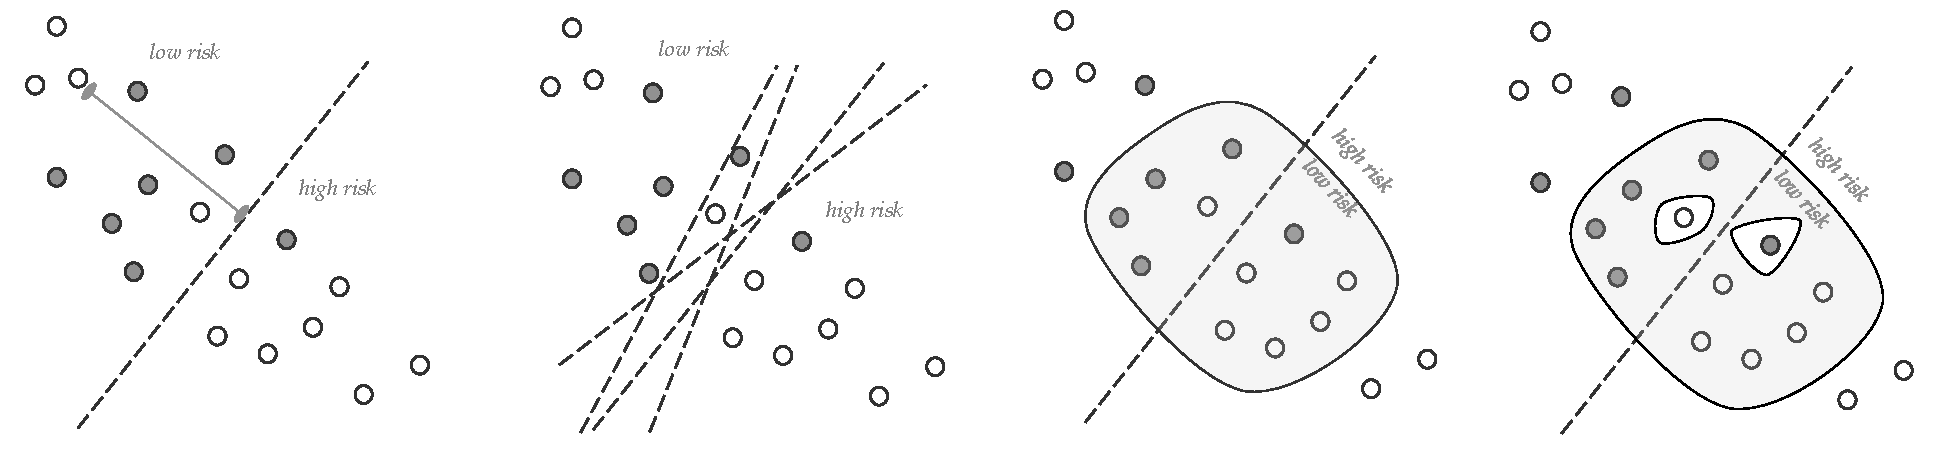
\includegraphics[width=\textwidth]{figures/active_learning.pdf}

\caption{A comparison of different query selection strategies for active learning on a non-stationary distribution. The shaded and empty circles are training data from two classes, $1$ and $0$ respectively. The red empty circles are samples from a new distribution (produced by executing the learned policy), and belong to class $0$. Typical strategies classify states close the decision boundary as risky(a), or for which a set of estimators disagree (b). Neither of these apply to our new samples in red. In contrast, we use a strategy that is amenable to non-stationary distributions by classifying  novel states as safe (i.e not risky) (c) and states in historically mislabeled regions. }
\label{fig:support_example}
\end{figure*}






\section{Problem Statement}
The goal of this work is to learn a policy that matches that of the supervisor's while asking the supervisor for as few examples as possible.

\mlnote{Ken is a big fan of  discussing the assumptions and model choices without notation before everything else, so a reader can quickly determine if this method suits there problem}

\noindent\textbf{Modeling Choices and Assumptions}  We model the system dynamics as markovian, stochastic, and stationary. Stationary meaning  given a state and a control the probability of the next state doesn't change over time. We model the initial state as sampled from a distribution over the state space.

We assume a known state space and set of controls. We assume access to a robot or simulator, such that we  can sample from the state sequences induced by a sequence of controls.   Lastly, we assume access to a supervisor who can, given a state, provide a control signal label. We assume the supervisor the supervisor can be noisy and imperfect, but also that the robot can at best reach the same level of performance of the supervisor after learning. 


\noindent\textbf{Policies and State Densities.}
We denote by $\mathcal{X}$ the set consisting of observable states for a robot task, consisting, for example, of \mlnote{We should discuss if we are going to consider images states or not}
high-dimensional vectors corresponding to images from a camera, or robot joint angles and object poses in the environment.
We furthermore consider a set $\mathcal{U}$ of allowable control inputs for the robot, which can be discrete or
continuous. We model dynamics, as Markovian, such that the probability of state $\mathbf{x_{t+1}}\in
\mathcal{X}$ can be determined from the previous state $\mathbf{x}_t\in\mathcal{X}$ and control input $\mathbf{u}_t\in
\mathcal{U}$: 
$$p(\bx_{t+1}|\bu_{t},\bx_{t}, \ldots, \bu_{0}, \bx_{0})=p(\bx_{t+1}|\bu_{t}, \bx_t)$$
We assume a probability density over initial states $p(\bx_0)$.
%We denote the probability density over the initial state also by $p:\mathcal{X}\to \mathbb{R}$. 

A trajectory $\hat{\tau}$ is a finite series of $T+1$ pairs of states visited and corresponding
control inputs at these states, $\hat{\tau} = (\mathbf{x}_0,\mathbf{u}_0, ...., \mathbf{x}_T,\mathbf{u}_T)$, where $\bx_t\in \mathcal{X}$
and $\bu_t\in \mathcal{U}$ for $t\in \{0, \ldots, T\}$ and some $T\in \mathbb{N}$.  
For a given trajectory $\hat{\tau}$ as above, we denote by ${\tau}$ the corresponding trajectory in state space,
${\tau} = (\bx_0,....,\bx_T)$.


A policy is a function $\pi: \mathcal{X} \to \mathcal{U}$ from states to control inputs. 
We consider a space of policies $\pi_{\theta}:\mathcal{X}\to \mathcal{U}$ parameterized by some $\theta\in \mathbb{R}^d$. Any such policy $\pi_{\theta}$ in an environment with probabilistic initial state density and Markovian dynamics
induces a density on trajectories of length $T+1$: $$p(\tau | \theta)=
p(\bx_0)\prod_{i=0}^{T-1}p(\bx_{t+1}|\pi_{\theta}(\bx_t),\bx_t)$$


Let $p(\bx_t|\theta)$ denote the value of the density of states visited at time $t$ if the robot follows the policy
$\pi_{\theta}$ from time $0$ to time $t-1$. This density can be computed by marginalization: $p(\bx_t|\theta) =
\int_{\bx_{t-1}}...\int_{\bx_1} p((\bx_t,...,\bx_1)|\theta) d\bx_{t-1}...d\bx_1$. Following \cite{ross2010reduction}, we can compute
the average density on states \emph{for any timepoint} by 
\begin{equation}
p(\bx|\theta) = \frac{1}{T} \sum^T_{t=1} p(\bx_t|\theta)
\label{eq:density}
\end{equation}


While we do not assume analytic knowledge of the distributions corresponding to: $p(\bx_{t+1}|\bx_t,\bu_t)$, $p(\bx_0)$, $p(\bx_t|
\theta)$ or $p(\bx|\theta)$, we assume that we have a stochastic real robot or a simulator such that for any state
$\bx_t$ and control $\bu_t$, we can sample the $\bx_{t+1}$ from the density $p(\bx_{t+1}|\pi_{\theta}(\bx_t),\bx_t)$. 
Therefore, when 'rolling out' trajectories under a policy
$\pi_{\theta}$, we utilize the robot or a simulator to sample the resulting stochastic trajectories rather than
estimating $p(\bx|\theta)$ itself.

\noindent\textbf{Objective.} The objective of  policy learning is to find a policy that minimizes some known cost function $C(\hat{\tau}) = \sum^T_{t=1} c(\bx_t,\bu_t)$ of a trajectory $\hat{\tau}$. The cost function $c:\mathcal{X}\times \mathcal{U}\to \mathbb{R}$ is typically user defined and task specific. 
For example, in the task of inserting a peg into a hole, a function on the distance between the peg's current and desired final state can
be considered \cite{levine2015end}.  

However in our learning from demonstration setup, the robot does not have access to the cost function itself. Instead, it only has access to 
a supervisor that we assume uses some $\tilde{\pi}$ to minimize $C(\hat{\tau})$, to an acceptable level. \mlnote{the last statement is intended to mean implementors of this algorithm have agreed that the supervisor may not be optimal, but has a level of performance that is worth automating} We are furthermore given
an initial set of $N$ stochastic demonstration trajectories $\lbrace \tilde{\tau}^1,...,\tilde{\tau}^N \rbrace$. 
which are the result of the supervisor applying this policy. This induces a training dataset $\mathcal{D}$ of all state-control input pairs from the demonstrated trajectories. 

We define a `surrogate' loss function $l:\mathcal{U}\times \mathcal{U}\to \mathbb{R}$, which provides a distance
measure between any pair of control values. In the continuous case, we consider $l(\bu_0,\bu_1) = ||\bu_0-\bu_1||^2$,
while in the discrete case $l(\bu_0,\bu_1) = 1$ if $\bu_0 \neq \bu_1$ and $l(\bu_0, \bu_1)=0$ otherwise.

Given a candidate policy $\pi_{\theta}$, we then use the surrogate loss function to approximately measure how "close" the policy's
returned control input $\pi_{\theta}(\bx)\in \mathcal{U}$ at a given state $\bx\in \mathcal{X}$ is to the supervisor's policy's control output
$\tilde{\pi}(\bx)\in \mathcal{U}$. The goal is to produce a policy that minimizes the surrgoate loss between relative to the supervisor's policy.


Following \cite{ross2010reduction}, our objective then consists of determining a policy $\pi_{\theta}$ minimizing the expected surrogate loss, where the expectation is taken over the distribution of states induced by the policy across any time point in the horizon:

 \vspace{-2ex}
\begin{align}\label{eq:LFD_obj}
\underset{\theta}{\min} \: E_{p(\bx|\theta)} [l(\pi_\theta(\bx),\tilde{\pi}(\bx))]
\end{align}
with $p(\bx|\theta)$ from Eq. \ref{eq:density}.

 If the robot could learn the policy  perfectly, this state density would match the one encountered in the user examples. But if the robot makes an error, that error changes the distribution of states that the robot will visit, which can lead to states that are far away from any examples and difficult to generalize to \cite{pomerleau1989alvinn}.Thus, motivating iterative algorithms like DAgger and now SHIV, which iterate between learning a policy and then the supervisor providing feedback. The feedback is in the form of control signals on states sampled from the robot's new distribution of states. 

% The optimization problem in Eq. \ref{eq:LFD_obj} is  typically non-convex. It can also be difficult to solve, since we only have access to samples from the supervisor's policy $\tilde{\pi}$ arising from the demonstration trajectories $\mathcal{D}$. To address these issues Stephane and Ross proposed an iterative method known as DAgger \cite{ross2010reduction}.

\section{SHIV} \label{sec:SHIV}

Both SHIV and DAgger \cite{ross2010reduction} solve the minimization in Eq. \ref{eq:LFD_obj} by iterating two steps: 1) compute a $\theta$ using the training data $\mathcal{D}$ thus far, and 2) execute the policy induced by the current $\theta$, and ask for labels for the encountered states. However, instead of querying the supervisor for every new state, SHIV actively decides whether the state is risky enough to warrant a query. 


\subsection{Step 1.}
The first step of any iteration $k$ is to compute a $\theta_k$ that minimizes surrogate loss on the current dataset $\mathcal{D}_k=\{(x_i,u_i)|i\in\{1,\ldots,M\}\}$ of demonstrated state-control pairs (initially just the set $\mathcal{D}$ of initial trajectory demonstrations):


 \vspace{-2ex}
\begin{align}\label{eq:super_objj}
\theta_{k} = \underset{\theta}{\argmin} \: \sum_{i=1}^{M} l(\pi_{\theta}(\bx_i),\bu_i).
\end{align}


This problem is a supervised learning problem, solvable by estimators like a support vector machine or a neural net \footnote{To handle the fact that the supervisor's policy can be noisy, a zero-mean noise term $\epsilon$ 
can be considered as present in the policy's output.  A regularization technique in the optimization is
used to control the smoothness of the function that is fit to the sampled data. In practice this regularization corresponds to a penalty term on either the L2 norm on the weights for regression based techniques or the slack coefficient for support vector machines \cite{scholkopf2002learning}.}.  Finding the right function representation and optimization method for a given problem is still an open question in machine learning. However a large number of advances have been made that make the use of these techniques very feasible \cite{scholkopf2002learning} \mlnote{The point was to acknowledge to traditional machine learning people that the problem is still hard and not solved. Ken didn't want to offend them}\adnote{is this really needed? what does it add? it basically says figuring out what method to use is hard; maybe say: performance will vary with the selection of a particular estimator \cite{}}
 

 \subsection{Step 2}
The second step starts in both SHIV and DAgger by rolling out the policy $\pi_{\theta_{k}}$ to sample states that are likely under $p(\bx|\theta_{k})$. 

What happens next, however, differs. For every state visited, DAgger requests the supervisor to provide the appropriate control/label. Formally, for a given sampled trajectory  $\hat{\tau} = (\bx_0,\bu_0,...,\bx_T,\bu_T )$, the supervisor provides labels $\tilde{\bu}_t$, where $\tilde{\bu}_t \sim \pi(\bx_t) + \epsilon$ for $t\in \{0, \ldots, T\}$.
The states and labeled controls are then aggregated into the next data set of demonstrations $\mathcal{D}_{k+1}$:
$$D_{k+1}=\mathcal{D}_k \cup \{(\bx_t,\tilde{\bu_t})\|t\in\{0,\ldots,T\}\} $$
%\fpnote{terms such as aggregated etc would be much clearer if we just refer to a particular line in the algorithm}

Providing correct control inputs or ``labeling'' for all states encountered at each
iteration can impose a large burden on the supervisor.
Instead of asking the supervisor for labels at all visited states $\{\bx_0,..,\bx_T\}$, SHIV uses a measure of risk to actively decide whether a label is necessary. For every state encountered $\bx_t$, it applies a decision function $g_{\sigma}$, which we introduce in the next section, parametrized by a risk-sensitivity parameter $\sigma$ which captures how smooth we expect the policy function to be: smoother functions imply that training examples have larger support, and data nearby will be less risky.

SHIV only asks for supervision on states for which $g_{\sigma}(\bx) \neq 0$: 


$$D_{k+1}=\mathcal{D}_k \cup \{(\bx_t,\tilde{\bu_t})\|t\in\{0,\ldots,T\},g(\bx_t)=-1\}$$

Steps 1 and 2 are repeated for $K$ iterations or until 
the cumulative surrogate is smaller than some predefined threshold\footnote{In the original DAgger the policy rolled out
was stochastically mixed with the supervisor, thus with probability $\beta$ it would either take the supervisor's action
or the robots. The use of this stochastically mix policy was for theoretical analysis. In practice, it is recommended
to set $\beta = 0$ to avoid biasing the sampling~\cite{NIPS2014_5421,ross2010reduction}}.


 For a conservative $\sigma$, the SHIV performance is analogous to DAgger without asking the expert when it is absolutely not necessary. However, if $\sigma$ is too high, then SHIV will not collect new data that is needed and revert back to the performance of offline methods. We analyze the dependence on $\sigma$ in Sec. \ref{sec:car}, and our results suggest that SHIV is robust to this parameter selection. 

\subsection{Measuring Risk}
% However, policy rollouts can in practice result in the robot entering dangerous states. For example, when DAgger was used on a
% quad-copter, the robot repeatedly crashed into trees before successfully learning to avoid them \cite{ross2013learning}.
We work under the assumption that a state can be risky for 2 reasons: 1) it lies in an area with a low density of
previously trained states, which can cause our policy to mis-predict the supervisor and incur high surrogate
loss \cite{tokdar2010importance}, or 2) the surrogate loss, or training error, of the current policy at a state in $\mathcal{D}$ is high, so that the state does not model the supervisor's control inputs correctly. 


To evaluate risk in high-dimensional state spaces (such as HOG features on images, like in our driving simulator, Fig. \ref{fig:teaser}(a)), we use
a modified version of the technique known as the One Class SVM that  approximately estimates a boundary of a user defined quantile of
a density representing the training data in $\mathcal{X}$ \cite{scholkopf2001estimating}.
%\fpnote{Refer to figure, replace "one way to do"  by "an approach to this problem is to" or similar - less informal}


%\subsection{Estimation of Quantile Level Sets}\label{sec:level}
We consider the problem of estimating the quantile level-sets of a distribution $P$ on a set $\mathcal{X}$ by means of a finite set of
independent and identically distributed samples $\mathbf{x}_1,...,\mathbf{x}_n\in \mathcal{X}$.
In most general terms, the quantile function for $P$ and subject to a class of measurable subsets $\mathcal{G}$ of $\mathcal{X}$ is
defined by
\begin{align}\label{eq:quantile}
U(\gamma) = \mbox{inf} \lbrace \lambda(G):P(G) \geq \gamma, G \in \mathcal{G} \rbrace \: 0<\gamma \leq 1
\end{align} 
$\lambda:\mathcal{G}\to \mathbb{R}$ above denotes a volume measure which most commonly is given by the Lebesgue measure.
Suppose furthermore that $G:[0,1]\to \mathcal{G}$ assigns a set $G(\gamma) \in \mathcal{G}$ that attains the infinum
measure (i.e. volume) for each $\gamma\in [0,1]$ (this set is in general not necessarily unique). 
$G(\gamma)$ denotes a set of minimum measure $G \in \mathcal{G}$ with $P(G(\gamma))\ge \gamma$. Note in particular that $G(1)$ is the support of the density $p$ corresponding to $P$, if $p$ exists. 

To handle distributions defined on high-dimensional spaces $\mathcal{X}$, work by Scholk{\"o}pf et al. looked at representing the class $\mathcal{G}$ via a kernel $k$ as the set of half-spaces in the support vector (SV) feature space \cite{scholkopf2001estimating}. 
By minimizing a support vector regularizer controlling the smoothness of the estimated level set function this work
derives an approximation of the quantile function described in Eq. \ref{eq:quantile}, which in particular has rigorous
convergence guarantees asymptotically when a normalized Gaussian kernel $k$ is chosen and bandwidths decay at an
appropriately chosen rate as the number of samples tends to infinity \cite{vert2006consistency}.
This approach can be thought of as employing $\lambda(G) = ||w||^2$, where $G_w = \lbrace x: f_w(x) \geq \rho \rbrace$,
$f_w(\mathbf{x}) = \sum_i w_i k(\mathbf{x}_i, \mathbf{x})$
and $(w,\rho)$ denote the weight vector and offset parameterizing a hyperplane in the feature space associated with a
Gaussian kernel $k(\bx_0,\bx_1) = e^{-||\bx_0 - \bx_1||^2/2\sigma^2}$.


Let $\Phi:\mathcal{X}\to \mathcal{F}$ denote the feature map corresponding to our exponential kernel, mapping the
observation space $\mathcal{X}$ into a Hilbert space $(\mathcal{F}, \langle, \rangle)$ such that $k(\bx, \bx') = \langle
\Phi(\bx), \Phi(\bx')\rangle$.

The One Class SVM proposed by \cite{scholkopf2001estimating} determines a hyperplane in feature space $\mathcal{F}$
maximally separating the input data from the origin:
\vspace{-2ex}
\begin{align}\label{eq:primal_sup}
    \underset{w\in \mathcal{F}, \mathbf{\xi} \in \mathbb{R}, \rho \in \mathbb{R}}{\mbox{minimize}}\: \frac{1}{2}||w||^2+\frac{1}{vn} \sum^n_i \xi_i - \rho\\
\mbox{s.t} \: \langle w,\Phi(x_i) \rangle \geq \rho - \xi_i, \: \xi_i \geq 0 \notag.
\end{align}

Here, the parameter $\nu$ controls the penalty or `slack term' and is equivalent to $\gamma$ \cite{vert2006consistency}
in the quantile definition, Eq. \ref{eq:quantile}, as the number of samples increases. The decision
function, determining point membership in the approximate quantile levelset is given by

\vspace{-2ex}
\begin{align}\label{eq:decision_func}
g(\bx) = \mbox{sgn}(\langle w,\Phi(x) \rangle-\rho).
\end{align}
\mlnote{The decison function actually used is not till the end, this is just a piece of it}
\adnote{we need $\sigma$ showing up here as $g_{\sigma}$ and remind the reader that the that inner product is a function of $\sigma$. might also be good to add a sentence or two on the intuitive role of sigma in this decision -- it captures how much we expect states to generalize, i.e. how smooth the policy function is}

Here, for $x\in \mathcal{X}$, $g(x)=0$ if $x$ lies on the quantile levelset,
$g(x) = 1$ if $x$ is strictly in the interior of the quantile super-levelset and $g(x) = -1$ 
if $x$ lies strictly in the quantile sub-levelset. The dual form of the optimization yields a Quadratic Program 
that can be solved efficiently \cite{scholkopf2001estimating}. In the dual the decision function is given by 

\vspace{-2ex}
\begin{align}
g(\bx) = \mbox{sgn}(\sum^N_{i=1}\alpha_i k(\bx_i,\bx)-\rho).
\end{align}

where $\alpha_i$ corresponds to the dual variables.  The novelty detection method can be visualized in Fig. \ref{fig:support_example}(c). 
However, even when sufficient data is available, the associated control inputs may be inconsistent or noisy and a resulting policy
optimizing Eq. \ref{eq:super_objj} may still incur a large surrogate loss. To account for this, we propose a
modification to the One Class SVM:

\begin{align}
y_i = \left\{
     \begin{array}{lr}
         1 & : l(\pi_{\theta}(\bx_i),\bu_i)\le \varepsilon\\
         -1 & : l(\pi_{\theta}(\bx_i),\bu_i)>\varepsilon
     \end{array}
   \right.
\end{align}

Where, in the case when $l$ denotes discrete $0-1$ loss, we set $\varepsilon = 0$, while in the continuous $L_2$ loss
case, $\varepsilon$ is a user defined threshold specifying allowable surrogate loss.
We use $y_i$ to modify the One Class SVM decision function as follows: 


We divide up our data in to two sets those correctly classified:
$$\mathcal{D}_{s}=\{\lbrace \bx_i,\bu_i \rbrace \in \mathcal{D}_{k}, y=1\}$$
and those states incorrectly classified: 
$$\mathcal{D}_{r}=\{\lbrace \bx_i,\bu_i \rbrace \in \mathcal{D}_{k}, y=-1\}$$
A separate One-Class SVM is then trained on each set of states, ($D_{s}$ and $D_{r}$) and providing measures of the level sets, $g_{s}$ and $g_{r}$. Specified by parameters $(\nu,\sigma)$ and $(\nu_r,\sigma_r)$, respectively. 

We then define the overall decision function as:

\vspace{-2ex}
\begin{align}\label{eq:decision_func}
g_{\sigma}(\bx) = g_{r} (\bx)+ g_{s}(\bx)
\end{align}

points are deemed risky if $g_{\sigma}(\bx) \neq 0$.  Practically, this modification corresponds to
`carving out holes' in the estimated quantile super-levelset such that neighborhoods around states with $y_i=-1$ are
excluded from the super-levelset. An illustration of this can be seen in Fig. \ref{fig:support_example}(d).

The decision function parametrization consists of the kernel bandwidth $\sigma$ in $g_s$. Changing sigma corresponds to how much influence each point in the training set has on the measure of risk. Large $\sigma$ corresponds to points nearby being safe. For a policy that is a smooth function $\sigma$ should be large. 

Our experiments analyze the performance of risk as a query selection strategy, with or without the addition of the second risk criteria, i.e. regions of space where the surrogate loss is high.



\section{Experiments}

We begin our experiments in an in-depth analysis of SHIV with a driving simulator. Here, we compare our query selection method with those typically used in active learning. We show that for a non-stationary state distribution like ours, the notion of risk based on novelty and misclassified regions performs better than a confidence and query-by-committee based methods. We continue with a sensitivity analysis, which suggests that the performance of SHIV is robust to the choice of how risky the robot is allowed to be (the $\sigma$ parameter from Eq. \ref{eq:decision_func}).

We then compare SHIV and DAgger on three domains: a driving simulator, push-grasping in clutter with a 4DOF arm, and surgery needle insertion using demonstrations from Dr. Douglas Boyd, a master surgeon at UC Davis. Each domain test different aspects of our algorithm: the driving simulator has a high dimensional visual state space, grasping in clutter has a human demonstrator provide the labels and is a challenging manipulation problem, surgical needle insertion uses data from a real robot and has an expert demonstrator. 

All experiments were run on a machine with OS X with a 2.7 GHz Intel core i7 processor and 16 GB
1600 MHz memory in Python 2.7. The policies, $\pi_\theta$ are either the linear SVM or  kernelized ridge regression classes in Scikit-Learn~\cite{scikit-learn}.

Our modified One Class SVM contains two different $\nu$ parameters, $\nu$ and $\nu_r$. We set $\nu = 0.1$ and $\nu_r =10^{-3}$ for all experiments. We tuned $\sigma$ and $\sigma_r$ by performing a grid search over different values on the surrogate loss for a single trial of SHIV for 3 iterations for each domain.


\subsection{SHIV Analysis}\label{sec:car}
We analyze our algorithm in a driving domain.

\noindent\textbf{Driving Simulator Domain.}
Our first domain is a common benchmark in Reinforcement Learning: learning a policy for a car to drive around a track~\cite{argall2009survey,ross2010efficient,ross2011reduction}. We implemented a driving simulator where the car must follow a polygonal track. We generated polygonal tracks by repeatedly sampling from a Gaussian with mean that is the center of the video game workspace centered in the middle of the workspace, and computing the convex hull of the sampled points.Then a convex hull is computed on the sampled points. In general this produces tracks composed of five to seven edges, an example is shown in Fig. \ref{fig:teaser}(a). If the car accidentally leaves the track, it is placed
back on the center of the track at a nearby position. The car's control input space is given by  $\mathcal{U} = \lbrace
-15^\circ, 0, 15^\circ \rbrace$. A control input instantly changes the angle of the car which drives at a unit speed. 
The internal state space of the car is given by the
xy-coordinates and the angle it is facing. In our experiments, the supervisor is provided by an algorithm that uses
state space search through the driving simulator to plan the next control. The algorithm is only allowed to search a finite amount a time ahead in the game and is prone to error, thus on averages crashes 5 times per lap. 

The supervisor drives around the track twice. We collect raw images of the simulation from a 2D bird's eye view
and use Gaussian Pyramids to down-sample the images to $125 \times 125$ RGB pixels and then extract Histogram of
Oriented Gradients (HOG) features using OpenCV. This results in a $27926$ dimensional state space description.
For both DAgger and \acro, we use a Linear Support Vector Machine (SVM) to parameterize allowable
policies $\pi_{\theta}$, with $\gamma=0.01$ as a regularization term on the slack variables, which was set via cross
validation on the initial training examples. We set SHIV's parameters  of the exponential kernel's bandwidth as $\sigma = 200$ and $\sigma_r = 200$.




\subsubsection{Comparison to active learning approaches.}\

\noindent\textbf{Independent Variables:} We compare four query selection methods. We compare our combined notion of risk (Fig. \ref{fig:support_example}(d)), with risk based on novelty alone (Fig. \ref{fig:support_example}(c)) in order to test whether carving out regions that have been misclassified previously is valuable. 

We also compare against two baselines, typically used in active learning. The first is confidence based on distance from the classification hyperplane \cite{tong2002support} (Fig. \ref{fig:support_example}(a)). We set the threshold distance to the average distance from the hyperplane for the mis-classified points in $\mathcal{D}_0$, which consisted of two demonstrations from our solver. 

The second baseline is Query By Committee (Fig. \ref{fig:support_example}(d)), which was trained via bagging \cite{breiman1996bagging}.  To obtain a committe, we divided the training data into 3 overlapping subsets, each with 80\% of the data. We trained a Linear SVM on each subset. If the three classifiers agreed with each other the point was determined low risk and if they disagree it was determined high risk. 
%We finally compared our combined risk approach against the traditional One Class SVM without the "carving out". 

We run each query selection method over 50 different car tracks.

\noindent\textbf{Dependent Measures. }We measured the percentage of truly risky states, encountered during the first policy roll out, that  are estimated to be safe by the active learning technique. The active learning techniques are trained on the initial demonstrations $\mathcal{D}_0$, which is different then the distribution being sampled from, $p(\bx|\theta_0)$, in this experiment.

\noindent\textbf{Results. } Fig. \ref{fig:active_comp}  plots the performance for each query selection method, averaged over 50 tracks. We observe a significant performance improvement with methods based on novelty compared to confidence and query by committee. Furthermore, using the combined measure of risk performs better than relying solely on novelty. 

\subsubsection{Sensitivity Analysis}. 

\noindent\textbf{Independent Variables.} To analyze the sensitivity of our method we varied the $\sigma$ parameter of the risk estimation function $g_{\sigma}$. $\sigma$ is a measure of how much risk we allow, with smaller $\sigma$s leading to more risk-adverse behavior. SHIV was ran for 6 iterations and averaged over 40 different randomized polygonal tracks. 

\noindent\textbf{Dependent Measures. } For each  $\sigma$, we measure the final cost function for the policy $\pi_{\theta}$ after 6 iterations and the number of examples SHIV requested from the supervisor. 

\noindent\textbf{Results. } As shown in Table \ref{tab:sens}, small $\sigma$, $\sigma = 1$, corresponds to always asking for help (many states labeled) and very large sigma, $\sigma = 350$, relates to  less data being used, but worse performance similar to the traditional (offline) supervised learning approaches. However, $\sigma$ values between $150$ and $250$ all achieve similarly good performance, suggesting that SHIV is robust to the choice of a particular $\sigma$.


\begin{table}[t]
\centering
\begin{tabular}{ R{2.5cm}||R{1.65cm}|R{1.65cm} }
 %\hline
 %\multicolumn{4}{|c|}{Sensitivity Analysis for Convergence to Best Grasp for Thompson sampling} \\
 %\hline 
 \hline
\specialcell{\bf Risk  Sensitivity ($\sigma$)} & \specialcell{\bf Final  Cost} & \specialcell{\bf States  Labeled} \\
 \hline
 1 & 6 & 4122 \\
 50 & 6 &  3864 \\
 150& 6 &  1859 \\
200 & 6 & 1524 \\
250 & 6 & 1536 \\
350 & 13 & 521\\

 %\hline
\end{tabular}
   \caption { \footnotesize  An analysis of the sensitivity of $\sigma$. SHIV was ran for 6 iterations and averaged over 40 different randomized polygonal tracks. Small $\sigma$, $\sigma = 1$, corresponds to always asking for help and very large sigma, $\sigma = 350$, relates to a lot less data being used, but worst performance similar to the traditional supervise learning approach. 
   }
		\tablabel{opt-p-comparison}
		\label{tab:sens}

\end{table}


\begin{figure}[t]
\centering
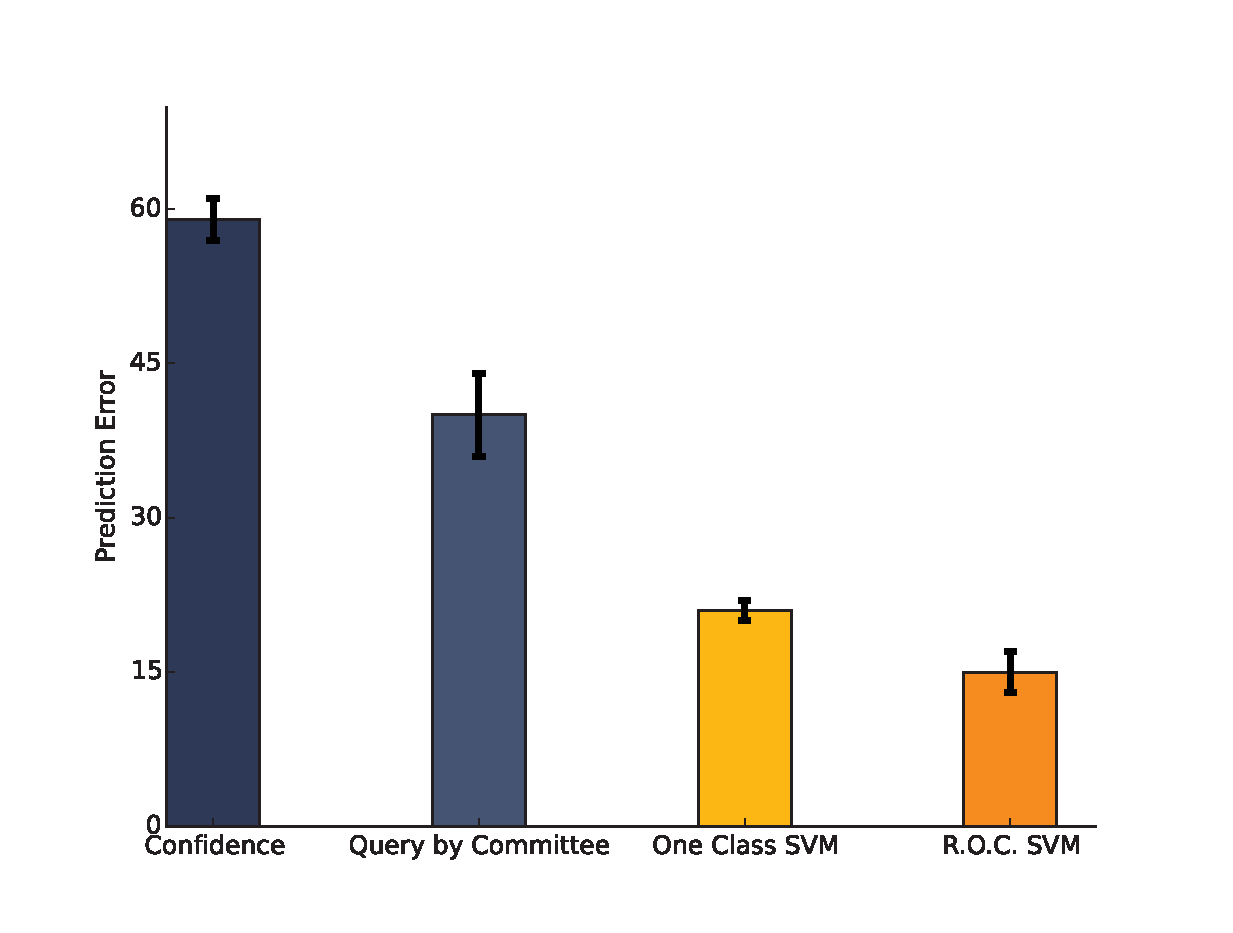
\includegraphics[width=\columnwidth, height=4cm]{figures/risk_bar.eps}
\caption {  A comparison of different active learning approaches in terms of the percentage of risky states that are estimated to be safe by the active learning technique during the first policy roll out. We compare against a confidence estimate of distance to hyperplane, query by committee for 3 hypothesis classifiers, the One Class SVM, and our modified One Class SVM.  Results  are averaged over 50 tracks and the policy $\pi_\theta$ is represented as a Linear SVM. 
   }

\label{fig:active_comp}
\end{figure}



\begin{figure}[t!]
\centering
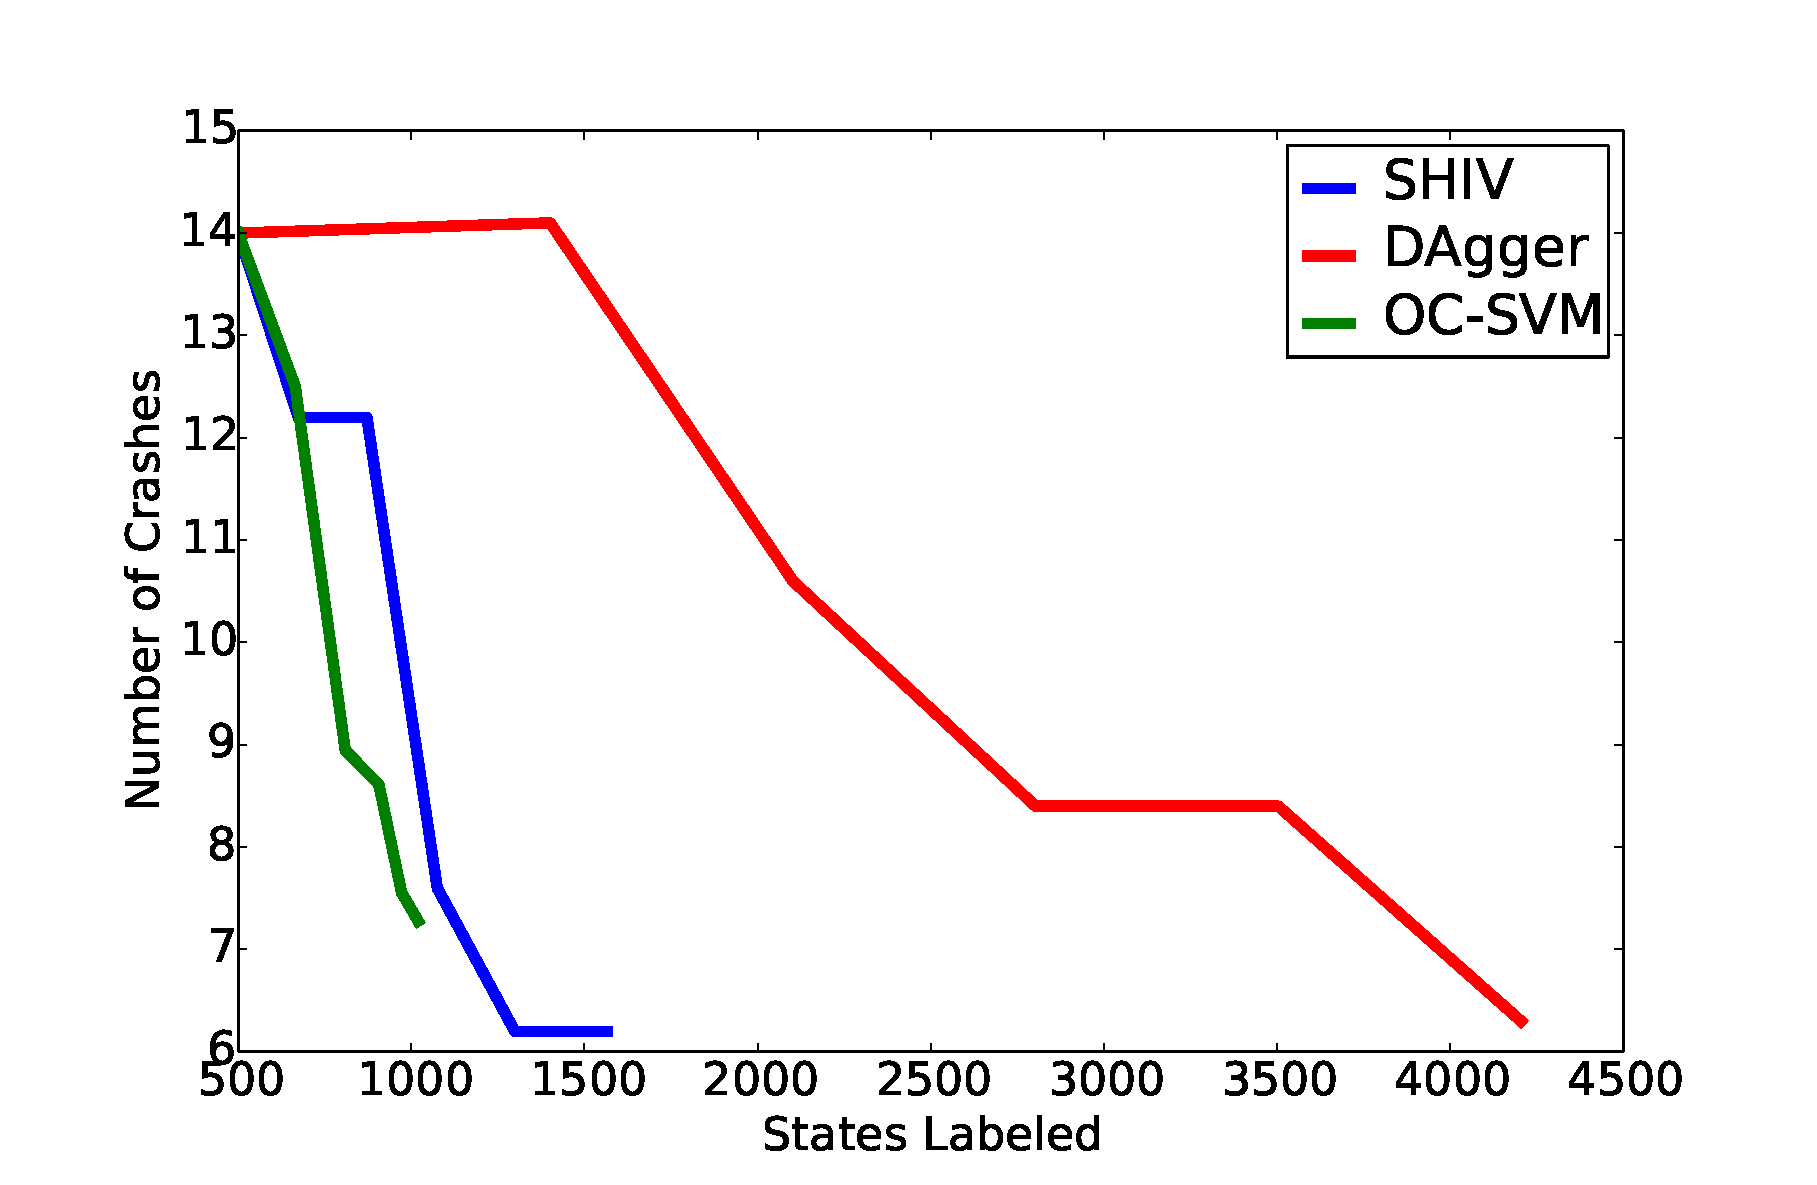
\includegraphics[width=\columnwidth, height=6cm]{figures/dagger_shiv_one_class.eps}
\caption{We compare performance for the Driving Simulator in terms of minimization of the underlying cost function $c(\bx,\bu)$, which is the  number of times the car left the track versus the number of queries made to the supervisor. In Fig. \ref{fig:car_cost}, we plot the performance of DAgger and SHIV.  Initial results, which are run for 6 iterations each and are averaged over 40 levels, shown in Fig. \ref{fig:car_cost} suggest an $71\%$ reduction in the number of queries needed for SHIV compared to DAgger,}
\vspace*{-10pt}
\label{fig:car_cost}
\end{figure}

\subsection{Comparing SHIV with DAgger}
We compare SHIV with DAgger on three domains: the driving simulator from above, push-grasping in clutter, and needle insertion.

\noindent\textbf{Independent Variables.} We manipulate two variables. First, we manipulate the online learning from demonstration algorithm we use: SHIV vs. DAgger. Second, we manipulate how many examples the algorithms are allowed to ask for: we set a budget of labeled states, and analyze performance as this budget increases.

\noindent\textbf{Dependent Measures.}For each algorithm and budget of states labeled, we measure the real cost that the learned policy attains (e.g. number of crashes in the driving domain).


\noindent\textbf{Hypothesis: } We expect SHIV to consistently achieve a lower cost that DAgger for the same budget of supervisor examples. Equivalently, we expect that SHIV achieves the same performance as DAgger, but by asking for fewer examples and thus reducing supervisor burden.

\subsubsection{Driving.}

\noindent\textbf{Domain.} Our first domain is the driving domain described above and illustrates SHIV's performance in high dimensions. 
We compare the policy's performance in terms of minimization of an underlying cost function $c(\bx,\bu)$, which is
defined to be total number of times the car left the track in relation to the number of queries made to the supervisor.

\noindent\textbf{Results.} 
In Fig. \ref{fig:car_cost}, we visualize the performance of DAgger and SHIV.  We run 6 iterations, which is a completion of both Step 1 and Step 2 described in Section \ref{sec:SHIV} of each algorithm over 40 different
randomized polygonal tracks. Figure \ref{fig:car_cost} presents averaged
results from these experiments, suggesting a $71\%$ reduction in the number of queries needed for SHIV compared to DAgger. 
 


\subsubsection{Grasping In Clutter}

\noindent\textbf{Domain.}
We investigate having a human demonstrator control a robot arm in 2D to reach a target object with out knocking other objects off a table. Grasping an object in a cluttered environment is a common task for a robot in an unstructured environment and has been considered a benchmark for robotic manipulation~ \cite{kitaevphysics,kingnonprehensile}. The task is difficult because modeling the physics of pushing an object is non-trivial and requires knowing the shape, mass distribution and friction coefficient of all objects on the table. We are interested in learning such a policy via human demonstrations. 

In lieu of real robot demonstrations, we used Box2D a physics simulator to model a virtual world. We simulate a 4 DOF robot arm with three main joints and a parallel jaw gripper as
displayed in Fig. \ref{fig:teaser}(b). SHIV and DAgger do not have access to the underlying dynamics of the simulator and must learn a policy from only demonstrations. 

For input the human demonstrator provides controls through an XBox controller. The right joystick was used to
    provide horizontal and vertical velocity inputs for the center of the end-effector which were then translated into
robot arm motions by means of a Jacobian transpose controller for the 3 main joint angles. The left `bumper' button on the joystick was used to provide a binary control signal to close the parallel jaw
gripper. The control inputs are hence modeled by the set $\mathcal{U} = \lbrace [-1,1],[-1,1],\lbrace 0,1 \rbrace \rbrace$.  

A state $\bx\in \mathcal{X}$ consisted of the 3 dimensional pose of the six objects on the table (translation and rotation), the 3 joint angles of the arm and a scalar value in the range $[0,1]$ that measured the position of the gripper, $1$ being fully closed and $0$ being opened. For our representation of $\pi_{\theta}$, we used kernelized ridge regression with the radial basis function as the kernel with the default Sci-Kit learn parameters. We defined the cost functions, $C(\bx,\bu)$, as the sum of the number of objects knocked off the table plus $10$ times the binary value indicating if the object is grasped or not. The order of magnitude difference in cost for grasping the object is to place emphasize on that portion of the task. The bandwidth parameters for SHIV were set to $\sigma_r = 5$ and $\sigma = 6$. For the $\epsilon$ term in the our risk method, we used the median in regression error which was the L2 distance between the predicted control and the true supervisor's control. 

In our experiment, a human demonstrator provided one demonstration and then iterated until the cost function was zero during the policy roll out. At each iteration, we sampled the pose of the target object from an isotropic Gaussian with a standard deviation that is equal to $3\%$ of the width of the table. 

\noindent\textbf{Results.} In Fig. \ref{fig:grasp_cost} , we show the cost function $c(\bx,\bu)$ averaged over 8 rounds for SHIV and DAgger. Supporting our hypothesis, our results suggests that SHIV can achieve the same performance with a 64\% reduction in the number of examples needed.

\begin{figure}[t!]
\centering
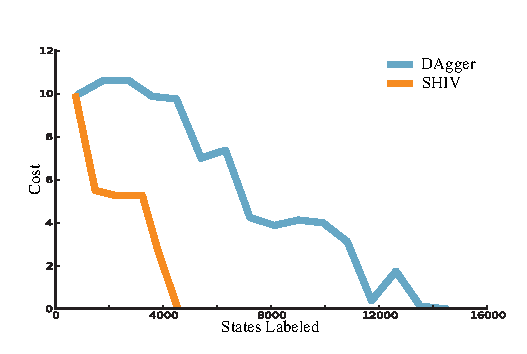
\includegraphics[width=\columnwidth, height=2in]{figures/grasp_clutter.eps}
\caption{We compare performance for Grasping in Clutter in terms of minimization of the underlying cost function $c(\bx,\bu)$, which is the sum of the number of objects knocked off the table plus 10 times the binary value indicating if the object is grasped or not. Initial results, which are averaged over 8 different trials suggest a $64\%$ reduction in the number of queries needed for SHIV compared to DAgger,}
\vspace*{-10pt}
\label{fig:grasp_cost}
\end{figure}




\subsubsection{Surgical Experiment}

\noindent\textbf{Domain.}
Robotic Surgical Assistants (RSAs) are frequently used for procedures such as: prostectomy, uterectomy, and tumorectomies within the abdominal and thoracic cavities with high success rates~\cite{van2013laparoscopic,darzi2004impact}. Currently, these devices are controlled by surgeons via physical tele-operation at all times; introducing autonomy of surgical sub-tasks has the potential to reduce cognitive load and facilitate supervised autonomy for remote tele-surgerical procedures.

Suture tying in surgery is a manually intensive task that can occur frequently through out a surgery. One important step
in suture tying is properly placing a needle in an initial configuration for insertion. Misplacement of this the needle
can lead to suture failure and potentially rupture the surrounding tissue \cite{liu2015optimal}. In this experiment, we
are interested in learning a policy to correct bad initial poses to the proper insertion pose as shown in Fig.
\ref{fig:support_example}. Dr. Douglas Boyd, a surgeon at UC Davis, provided us with a collection of demonstrations on a Intuitive Surgical Da Vinci Research Kit \cite{AnnualReport2014}.

Dr. Boyd demonstrated a series of trajectories that each started at an initial attempted needle insertion pose $P_0$ and
applied the necessary corrections to achieve a goal pose $P_G$. The time horizon, $T$ of each trajectory was on average 80.  We used three of these demonstrations as our initial
dataset $\mathcal{D}_0$, thus $|\mathcal{D}_0| = 240$. In order to study convergence of both SHIV and DAgger, we chose to create a synthetic expert for online learning part. The expert controller computed the transformation between the desired insertion pose and the current pose  by calculating the inverse of a transformation matrix, $C = P_0P_G^{-1}$. Then converted $C$ to the associated lie algebra vector $c \in \mathbb{R}^6$ for $SE(3)$ and normalize it to the average magnitude of the control,  $||\bar{c}_D||$, Doug Boyd applied to the robot. 

The policy $\pi_{\theta}$ was represented as kernel ridge regression with the default values given in Sci-Kit learn. The state $\mathcal{X}$ was  a 16 dimensional vector consisting of the elements in the pose $P$ vector. The control space $\mathcal{U}$ was a $\mathbb{R}^6$ vector representing the Lie algebra. 

For the $\epsilon$ term in the our risk method, we used the median in regression error which was the L2 distance between the predicted control and the true supervisor's control. 
regions respectively. The bandwidth, $\sigma$, in the rbf kernel was set to $2$ and $\sigma_b = 1$.

For trials we sample a start position from a Gaussian on the translational component of $P_0$ with isotropic variance of
$0.1$ cm. The distance between initial $P_0$ and $P_G$ is roughly $3$ cm. Our cost function $c(\bx,\bu)$ is measured in
terms of Euclidean distance in translational component, which is in centimeters. We run DAgger and SHIV both for 20 iterations and average over 40 different starting positions.

\noindent\textbf{Results. }
 In Fig. \ref{fig:grasp_cost} , we show the cost function $c(\bx,\bu)$ averaged over 40 rounds for SHIV and DAgger. Supporting our hypothesis, our results suggests that SHIV can achieve the same performance with a $67\%$ reduction in the number of examples needed.






\begin{figure}[t!]
\centering
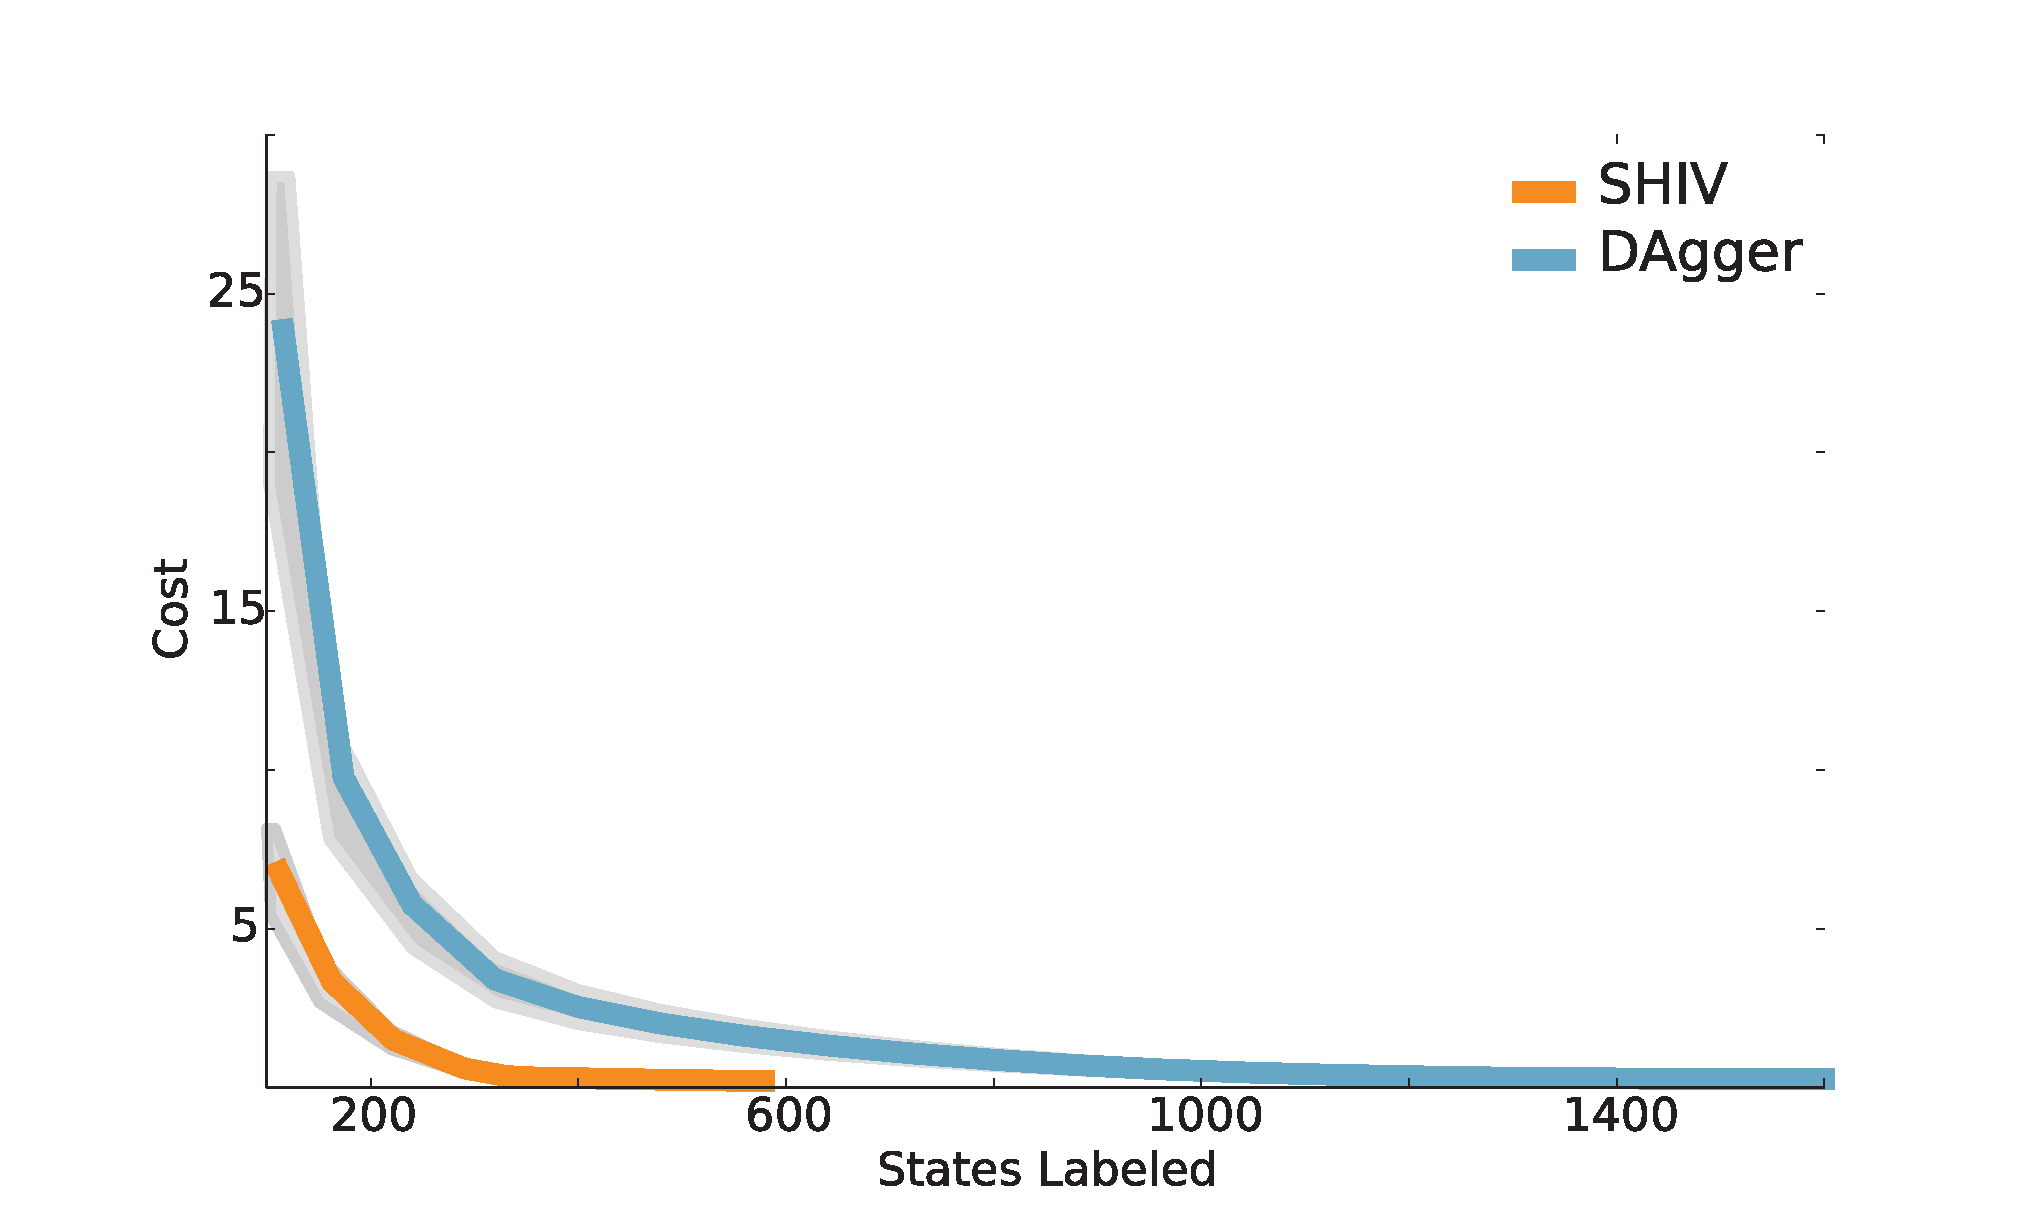
\includegraphics[width=\columnwidth, height=2in]{figures/needle_insertion_results.eps}
\caption{We compare performance in terms of minimization of the underlying cost function $c(\bx,\bu)$, which is euclidean distance between translation in centimeters. In Fig. \ref{fig:car_cost}, we plot the performance of DAgger and SHIV without the modification.  Initial results, which are run for 20 iterations each and are averaged over 40 different initial starting positions, shown in Fig. \ref{fig:car_cost} suggest an $67\%$ reduction in the number of queries needed for SHIV compared to DAgger,}
\vspace*{-10pt}
\label{fig:needle}
\end{figure}



\section{Discussions and Future Work}
Online imitation learning algorithms have been successful on array of task~\cite{NIPS2014_5421,ross2010reduction}, however can significantly increase the burden on a supervisor. Our algorithm, SHIV, implements stream-based active learning with a query selection method that evaluates risk in a manner tailored to non-stationary state distributions. We empirically evaluated our method on three different domains: a driving simulator, grasping in clutter and surgical needle insertion. Results suggest a $70\%$ reduction in the number of queries to the supervisor needed. 

While achieving a high level of performance, SHIV has several limitations. For instance, the selection of the value of $\sigma$ can affect performance and a poor choice could result in the algorithm becoming offline imitation learning, as shown in Table \ref{tab:sens}. Future work will look at better understanding the relationship of $\sigma$ to the function $\pi_{\theta}$ and how to automatically select it. 

 Furthermore, to update the decision function $g_{\sigma}$ requires solving a quadratic program, which has an upper bound computationally complexity of $O(n^3)$ in the number of data points. This can effect the ability of using our modified One Class SVM for larger problems. Future work will look at using techniques such as random features or PCA on the kernel Gram matrix to allow for better scaling~\cite{scholkopf2002learning}.
 
 Lastly, online imitation learning only allows a policy to learn to be as good as the supervisor. If the supervisor is imperfect then the robot will be as well. Future work will look at combining techniques from inverse reinforcment learning\cite{argall2009survey} with online imitation learning to allow the robot to improve upon it's policy after supervision is done. 
 

\section{Acknowledgments} 
\fpnote{remove in the initial submission if we are pressed for space}
This work is supported in part by the U.S. National Science Foundation under Award IIS-1227536 and NSF-Graduate Research Fellowship.. 
We thank UC Berkeley and our colleagues who gave feedback and suggestions, in particular Sanjay Krishnan, Siddarth Sen, Steve McKinley, Sachin Patil and Sergey Levine.




\bibliographystyle{IEEEtranS}
\bibliography{references}



\end{document}
